\cleartooddpage[\thispagestyle{empty}]
\chapter{Veritas}

\begin{figure}[h]
  \begin{center}
    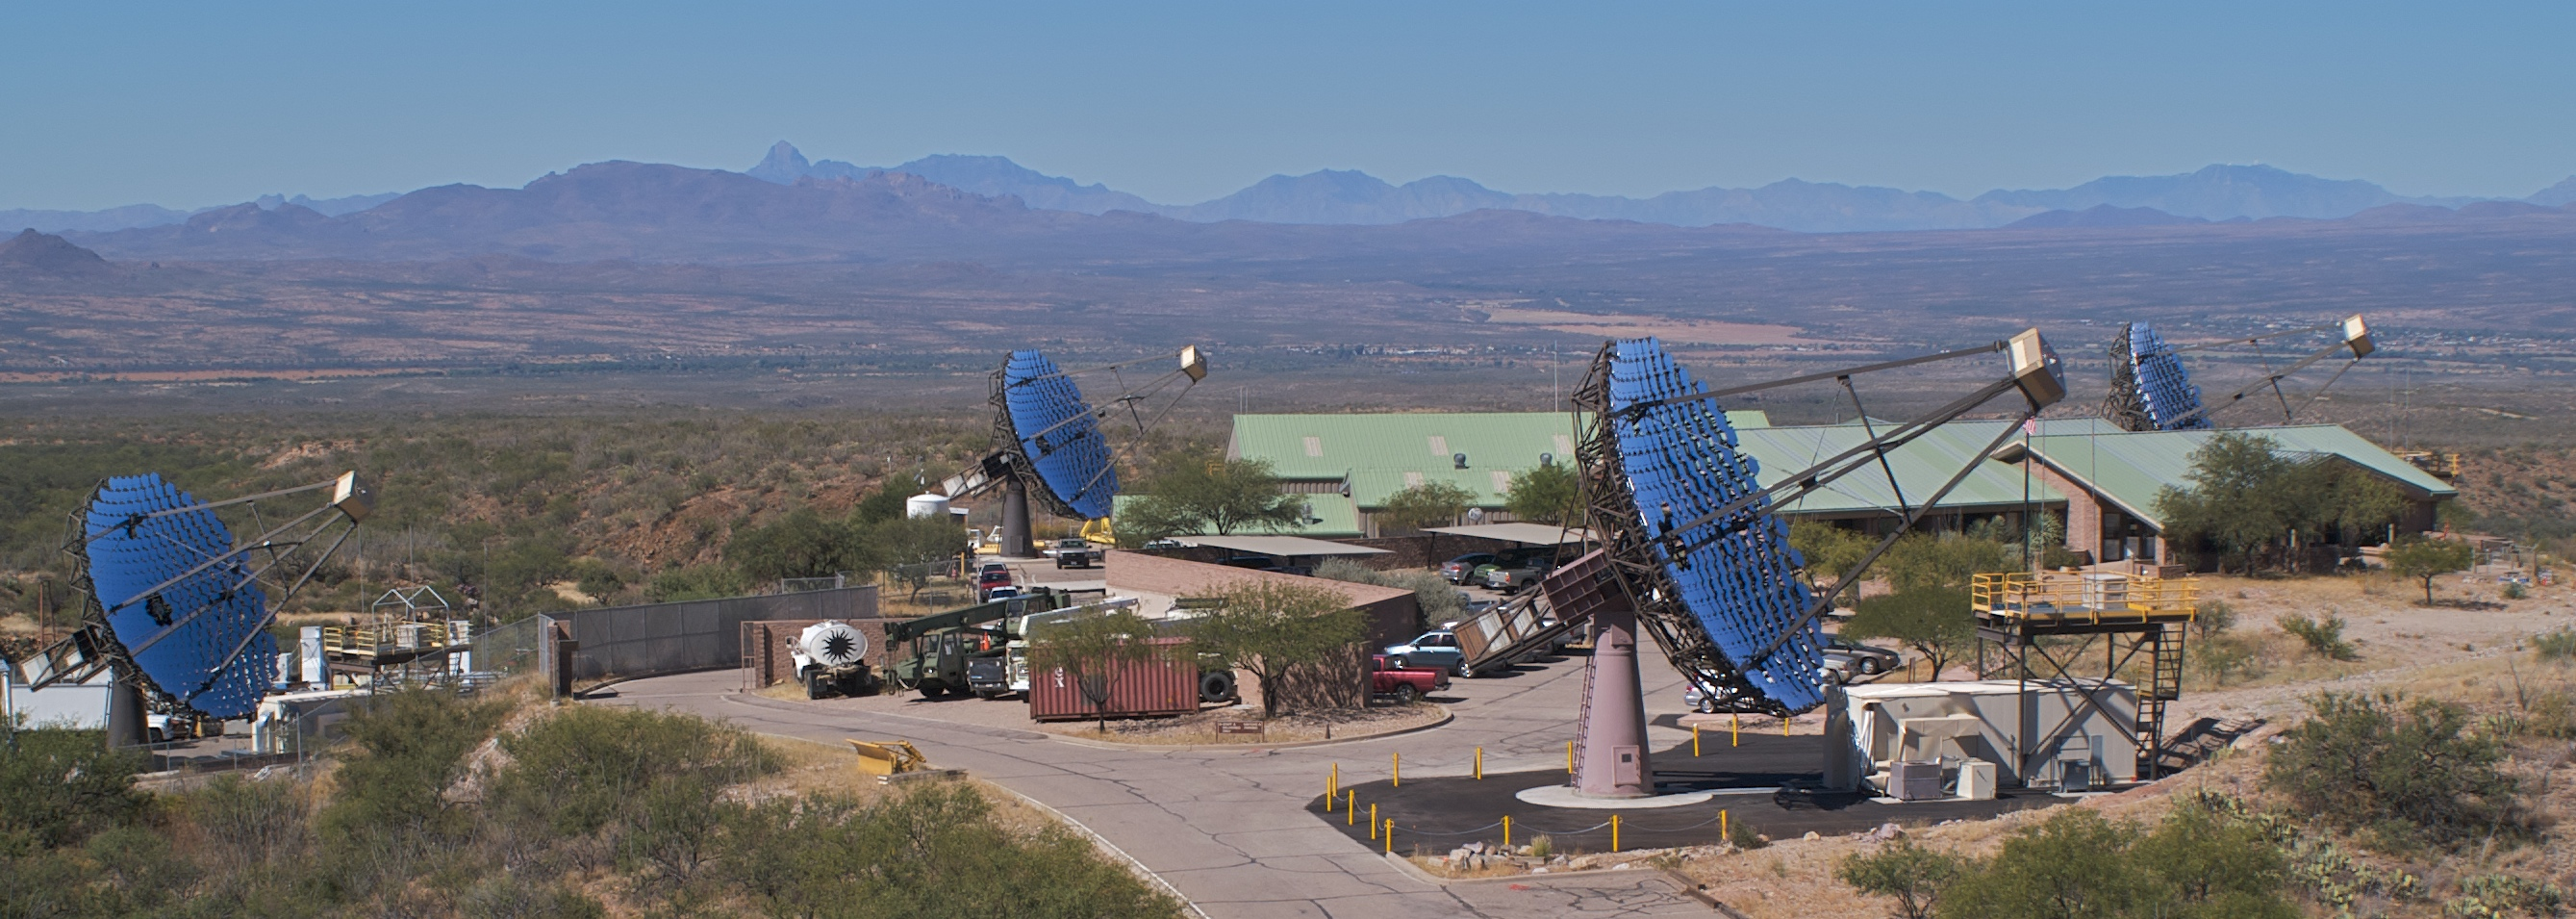
\includegraphics[width=0.95\textwidth]{images/veritas_array_v6}
    \caption[VERITAS Array]{The VERITAS observatory.}\label{fig:veritasarray}
  \end{center}
\end{figure}

VERITAS is an arrary of four Imaging Atmospheric Cherenkov Telescopes, each spaced $\nicetilde50m$ apart.
Each telescope possesses an array of 345 mirrors, and a 499-Photomultiplier-Tube camera out on a set of four struts, called quads.
Each mirror focuses photons onto the camera.
In Section \ref{sec:hardware}, the different hardware components are discussed.
In Section \ref{sec:trig}, the different trigger levels are discussed.
The methods for image reconstruction are discussed in Section \ref{sec:imgrecon}.
In Section \ref{sec:recon}, the reconstruction used in different parts of the analysis are discussed, including the per-telescope image reconstruction in Subsection \ref{subsec:imgrecon}, the direction reconstruction in Subsection \ref{subsec:posrecon}, and the energy reconstruction in Subsection \ref{subsec:enrecon}.


\section{Hardware}\label{sec:hardware}
When a gamma-ray produces an air shower in the atmosphere, the shower emits numerous Cherenkov photons, over a time period of nanoseconds.
When the light from the shower reaches the telescopes, only a handful of Cherenkov photons remain, and these photons are spread out over several nanoseconds.

To detect these individual Cherenkov photons, Photomultiplier tubes are used to amplify the signal from single photons.
This produces an analog voltage pulse that then must be digitized.
As the voltage pulses widths must be \nicetilde{}ns to prevent overlapping with other showers, the digization hardware measures each voltage pulse in 1-nanosecond-wide(??) time bins.
Though faint showers may only posess a few photons, brighter showers can still shine several thousand photons onto individual pixels.
This means that the digization hardware must be able to handle a large dynamic range of inputs, over several orders of magnitude.
To accomplish this, two amplification levels are used in the digization circuit, High Gain for voltage pulses of a few photons, and Low Gain for voltage pulses of several thousand photons.

\subsection{Telescope Pointing}

\begin{figure}[h]
  \begin{center}
    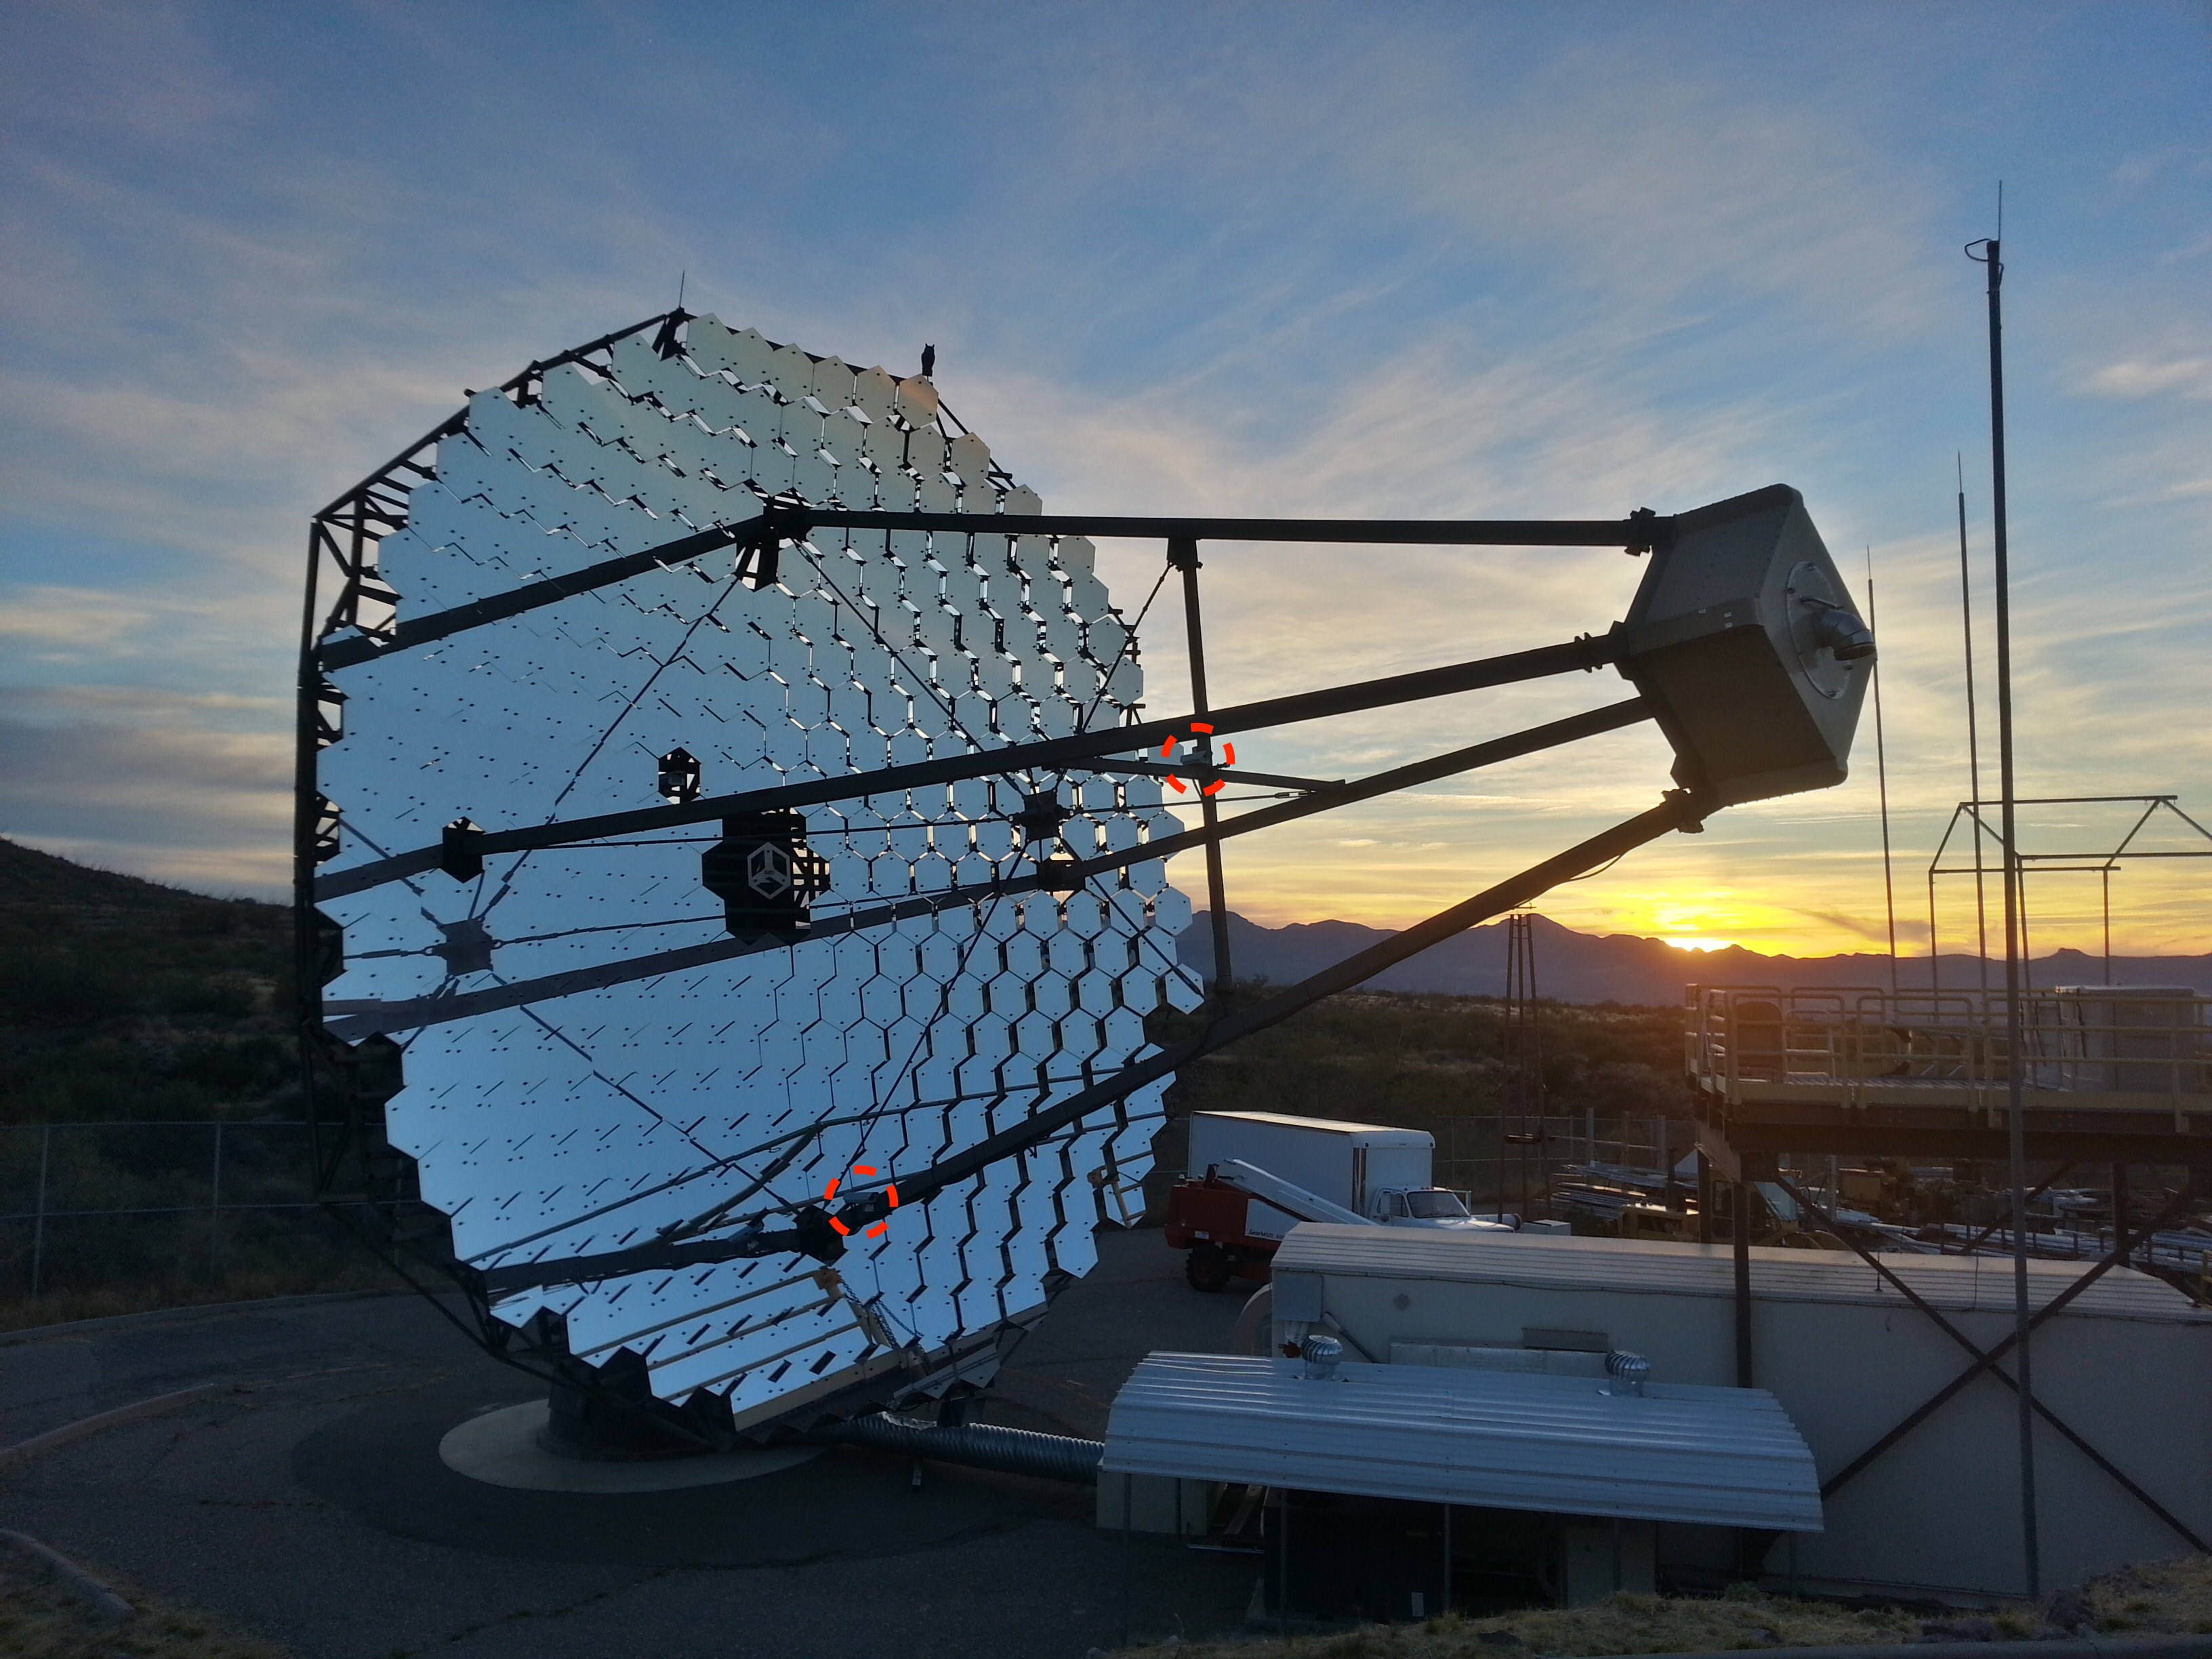
\includegraphics[width=0.95\textwidth]{images/single_telescope}
    \caption[Single Telescope]{View of the 345 mirrors, the support structure, and the PMT Camera housing at the end of the four supporting arms.}\label{fig:davcottel}
  \end{center}
\end{figure}

Like most telescopes, each VERITAS telescope has an immobile base fixed to the ground, and a pointable dish for collecting light.
This dish can rotate in azimuth and in elevation, with enough range in both axes to point at any direction above the horizon.
At their fastest, the telescopes can slew at a rate of 1\degree per second.
To track where the telescopes are pointing, the motors that drive the azimuth and elevation movement have encoders that digitize the pointing direction of the dishes.
However, as the dishes are large metal structures, they bend and flex at different elevations and azimuths.
To account for this flexing, the encoder values are then given to a structural model (??), which accounts for the dish structure bending at different azimuths and elevations.
After applying this model, the telescope pointing can be tracked with an accuracy of 0.013\degree to 0.027\degree \cite{Veritas_Detector}.

As an improvement to the encoder measurement, a Virtual Pointing Monitor (VPM) system is also in place.
The VPM consists of two CCD cameras fixed to each telescope, pointing parallel to the telescope pointing, and a set of LED lights attached to the camera, next to the Winston cones (see section \ref{sec:pmts}).
The first CCD camera is attached below the bottom mirrors, and images the stars in the field of view.
The second CCD camera is attached to the support struts, roughly halfway between the mirrors and the camera, and images the focal plane of the telescope.
Both cameras are visible in figure \ref{fig:davcottel}
During regular observations, these cameras take images of the background stars and the focal plane every two seconds, and (??), resulting in an improved pointing accuracy of \nicetilde 0.0069\degree (originally in griffen thesis 2016, pg45, but is there a better citation??).

As the VERITAS telescopes are based on old designs for a military solar concentrator that sets targets on fire\cite{daviescotton}, the VERITAS telescopes have similar abilities.
This mostly means that care must be taken during the day to point the telescopes away from the sun during maintanance and storage.
% 100m^2 * 1000w/m^2 = 100,000W
If any direct sunlight falls onto the telscope mirrors, the \nicetilde100,000 Watts of light will be concentrated either onto the camera, or a point within a few meters of the camera, which could potentially cause signficant damage to the telescope hardware or nearby plants, animals, and people.
VERITAS telescopes are stored during the day by pointing them at \nicetilde0\degree elevation, North.


\subsection{Mirrors}

When cherenkov light first interacts with the telescope array, it is by being reflected by one of 345 mirrors.
These mirrors face towards the incoming cherenkov light, with the PMTs positioned in a camera box, facing the mirrors, shown in figure \ref{fig:davcottel}.
This configuration is referred to as a Davies-Cotton telescope \cite{daviescotton}.
Each mirror has an area of 0.322$m^2$, and a spherical curvature radius of 24m.
The mirrors are each mounted along the support structure so that the total diameter of the telescope mirror area is 12m, with a focal length of 12m, and a total mirror area of 111$m^2$ \cite{Veritas_Detector}.
The mirrors' reflectivity as a function of wavelength is shown in figure \ref{fig:mirreflect}.

\begin{figure}[h]
  \begin{center}
    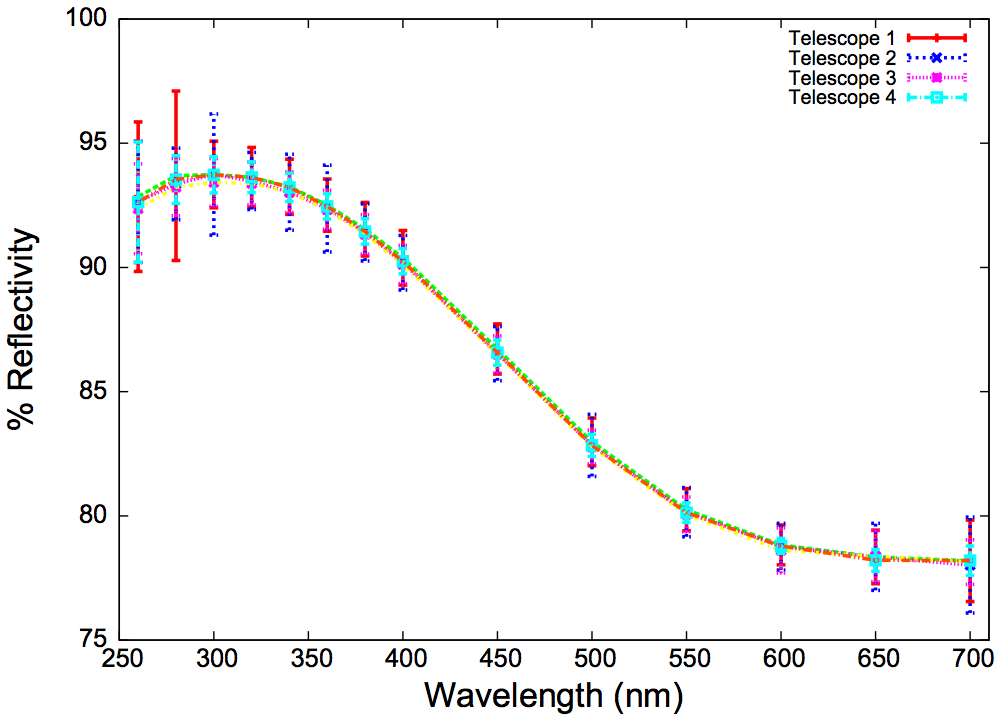
\includegraphics[width=0.75\textwidth]{images/mirror_reflect}
    \caption[Mirror Reflectivity]{Mirror reflectivity as a function of wavelength for each telescope, from \cite{mirrorfacets}.  The VERITAS specifications state that the mirror reflectivity must be $\geq 85\%$ between 280nm and 450nm.}\label{fig:mirreflect}
  \end{center}
\end{figure}

As the mirrors are exposed to the elements, they slowly accumulate dust and scratches.
To combat this, they are cleaned and recoated at regular (yearly??) intervals.
Each mirror is attached to the support structure via three adjustable mounting points, meaning the mirror orientation can be adjusted to point directly on the camera, detailed in \cite{mirroralign}.
This alignment is measured and adjusted at regular intervals, using background stars as a calibration source??.


\subsubsection{Mirror Alignment}

\subsubsection{Star Point Spread Function}


\subsection{PMTs}\label{sec:pmts}

Each telescope has a PMT Camera on the end of four supporting arms, inside a protective housing.
This camera consists of 499 Photo Multiplier Tubes (PMTs), each with a Winston cone to increase the light collection area for each PMT.
The PMTs are Hamamatsu's model R10560-100-20 MOD \cite{pmtmodels}.
These winston cones can be seen attached to the PMTs in figure \ref{fig:winstcones}.

\begin{figure}[h]
  \begin{center}
    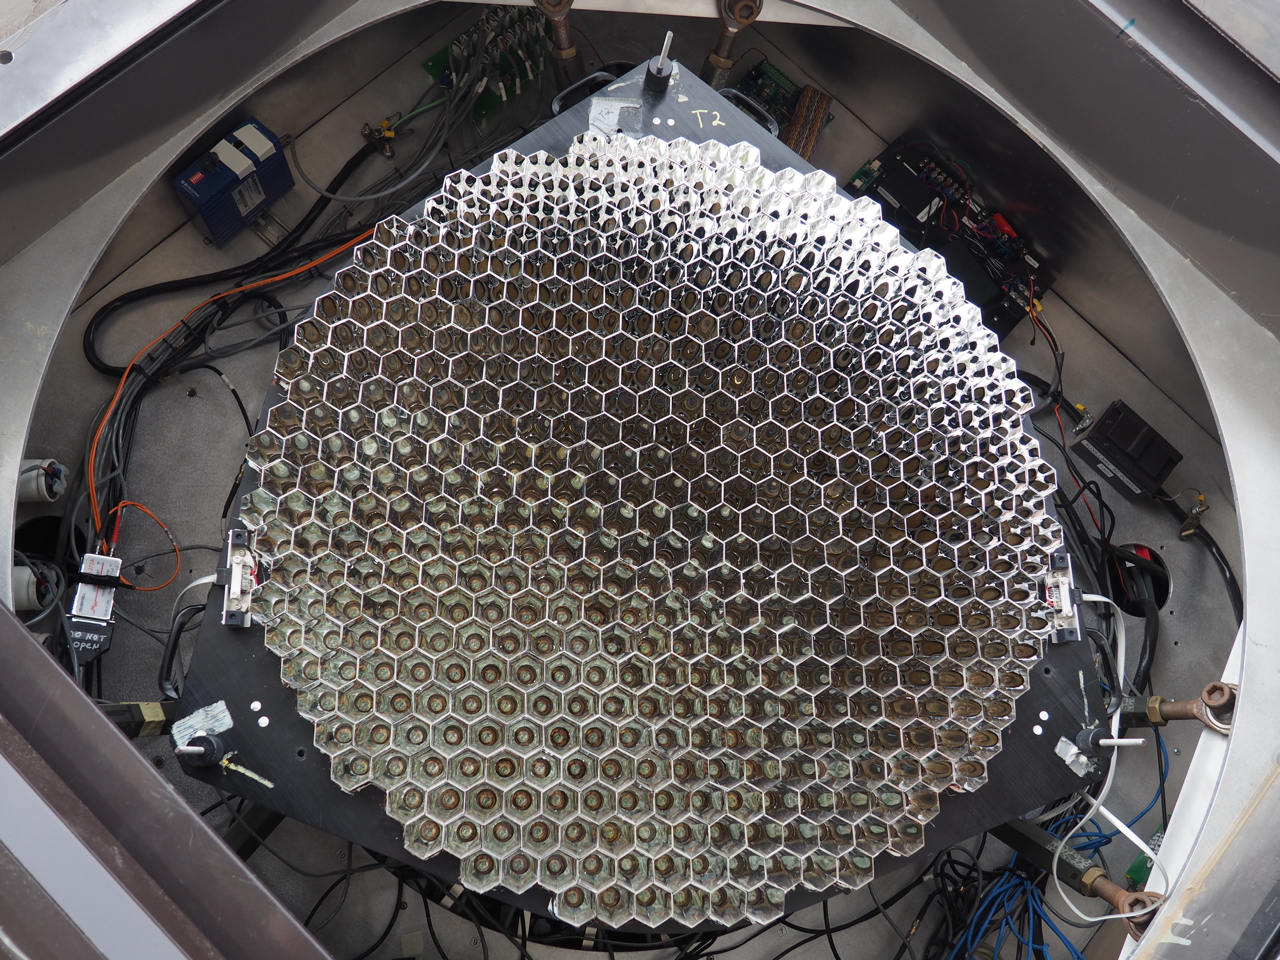
\includegraphics[width=0.75\textwidth]{images/winston_cones_t2}
    \caption[Winston Cones]{Hexagonal Winston cones over the circular PMTs, inside the camera housing.}\label{fig:winstcones}
  \end{center}
\end{figure}

To operate, the PMTs are connected to high voltage, which is typically around several hundred Volts.

\begin{figure}[h]
  \begin{center}
    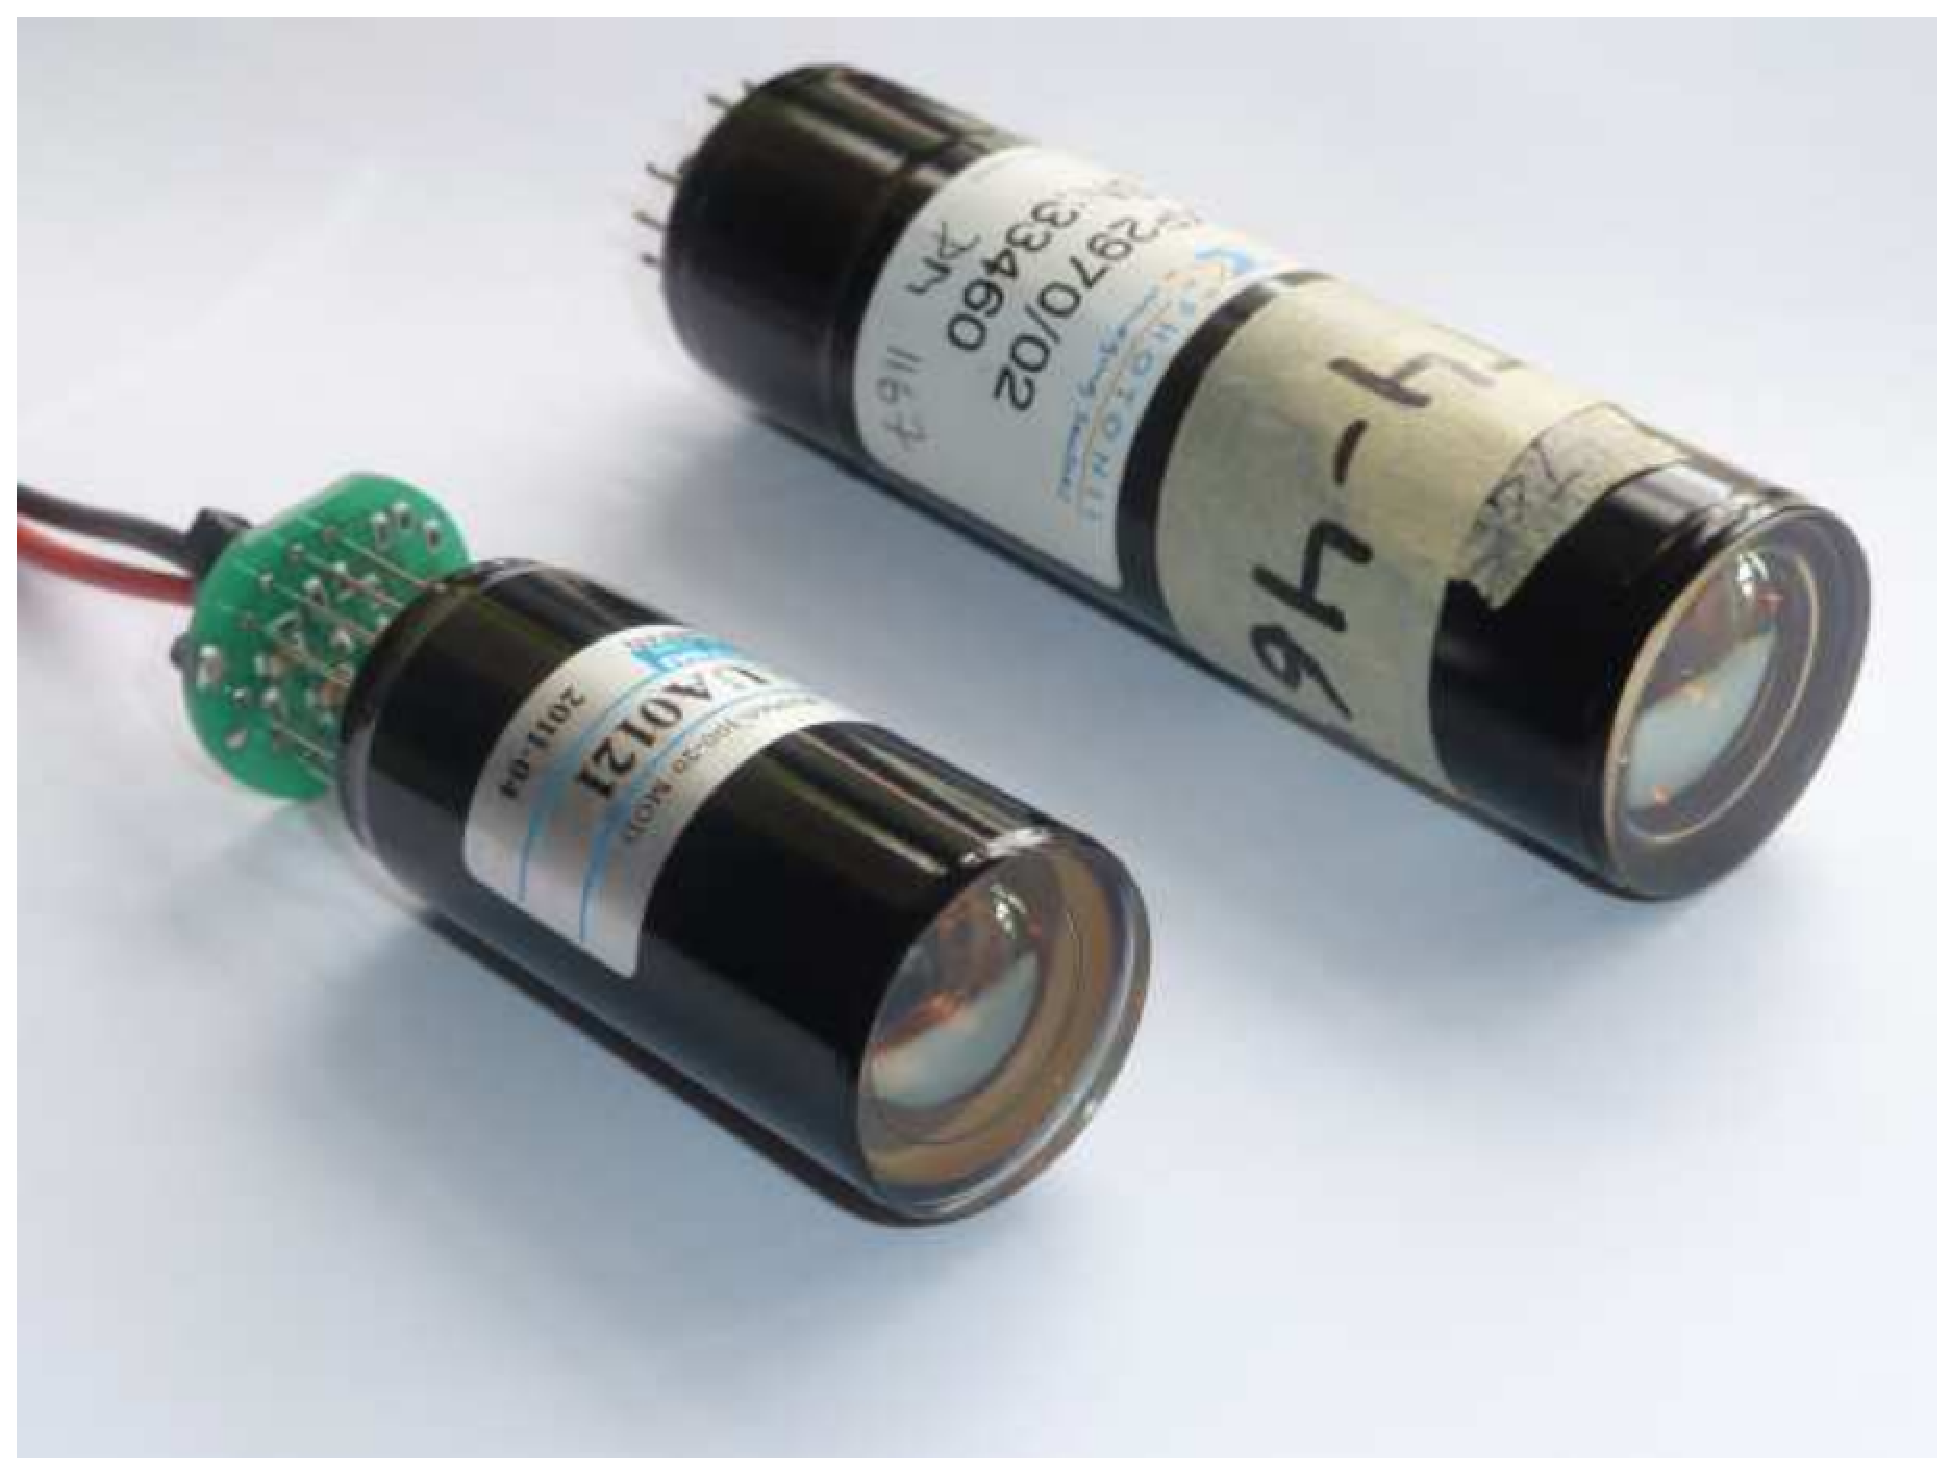
\includegraphics[width=0.75\textwidth]{images/pmt_models}
    \caption[PMT Models]{The two PMT models used in the VERITAS cameras. \cite{pmtmodels}}\label{fig:pmtmodels}
  \end{center}
\end{figure}

The PMTs' output signals are first sent through an amplifier, before travelling down a \nicetilde45m (cite??) cable to electronics stationed near the telescope.
The electronics then digitize the signal.

The first circuit that the signal passes through is a Constant Fraction Descriminator (CFD) circuit.
This circuit duplicates the signal voltage pulse from the PMTs, inverts and delays the duplicate pulse, and adds it back to the original pulse.
This combined pulse then crosses the zero-volts threshold (called a Zero Threshold Descriminator) at the same time (how 'same'?? within 1 ns??) as the original pulse reaches its peak, acting as a maximum-voltage detection circuit.
When a maximum voltage is detected by the circuit, it emits a 10ns trigger pulse to other electronics.

The use of this circuit has two main benefits.
The first use is that the CFD circuit will trigger at the same time regardless of the pulse size (??).
If a simple threshold trigger is used to detect a signal pulse, the time of the trigger will be earlier for larger pulses, and later for smaller pulses.
The CFD's zero threshold trigger time is around the time when the signal voltage pulse is at 75\% of its maximum value. (cite??)

The second use is that when the CFD circuit detects a voltage pulse larger than a given maximum threshold, it can emit an extra logic trigger, called a low-gain trigger.
This extra low-gain trigger can then be used by later electronics to determine the rough size of the original signal voltage pulse.

CFD behavior cite??

CFD model??

FADC model??

After the CFD emits a trigger pulse, the signal voltage pulse is passed to another circuit for digization, a Flash Analog-to-Digital Circuit, or FADC.
This FADC circuit then, for each nanosecond time bin, measures how large the voltage pulse is with a series of 255 (??) constant-voltage thresholds.
The highest threshold that is crossed in a single time bin then determines the digital voltage value that is saved to the FADC buffer for that time bin.

If the low-gain trigger pulse was also recieved by the FADC, then the signal voltage pulse is de-amplified before being digitized, since the CFD low-gain threshold is set to lower than the FADC maximum digitizable voltage.
If this low-gain triggering did not take place, then the FADC would become saturated, which effectivly hides how large the voltage pulse actually is.
Once the voltage pulse is digitized, it is saved to a rolling buffer (how long is the buffer??) in the FADC, waiting for other future triggers to occur.

\subsubsection{PMT Upgrade}
In summer of 2012, all PMTs in the telescopes were replaced with improved PMTs.
Specifically, the original Photonis XP2970 models were replaced with the Hamamatsu R10560-100-20 MOD.
This was done because that R10560 has a considerably higher quantum efficiency (\nicetilde$90\%$), compared to the XP2970 (\nicetilde$75\%$).
This higher quantum efficiency means more photons from a shower are detected by the PMT, which means VERITAS is more sensitive to lower energy gamma rays\cite{pmtmodels}.

The data used in this thesis was taken both before and the upgrade, which means the telescope performance is different for these two time periods.
This is accounted for by separate simulations for each PMT type, mostly resulting in different effective areas at the lower energies.(check!??)


\subsubsection{PMT Gain Flatfielding}

The VERITAS PMTs are all the same model, but there are still differences from PMT to PMT.
These differences cause the same number of input photons to create differently-shaped output signal voltage pulses.
To account for this, the high voltage of individual(??) PMTs can be varied, so that their pulse shapes are as similar as possible.
Doing this is called Gain Flatfielding.

This is performed by (??)

\subsection{Triggers}\label{sec:trig}

The operation of VERITAS requires digitizing voltage pulses once per nanosecond, per photomultiplier tube.
This means that, with 255 voltage levels, 1 second of raw voltage data would require 2 Terabytes of space.
As this is unfeasable with today's computing systems, only subsets of the raw pixel voltages can be saved.
Thus, VERITAS has a system where the raw data is only saved when certain triggers are met.

Initially, all voltage pulses are binned in time, and each time bin is copied to a buffer on a fast electronics board ??.
The board then goes through several trigger layers.

The L1 trigger is met when multiple time-binned voltage measurements in a single pixel combine to cross a specified threshold voltage.
At the single pixel level, the signals that are preferred are from multiple photons, close in time.
The background signals that are rejected by this trigger include voltage pulses from ambient photons from the night sky background (NSB) and from human-reproduced background photons (cars, streetlights, illuminated clouds, etc.).
When a pixel's L1 trigger is met, this signal is sent to the L2 trigger system.

The L2 trigger is invoked when several adjacent pixels produce an L1 trigger within a span of several of nanoseconds.
This image trigger, when met, is then sent to the L3 trigger system.

The L3 trigger is invoked when two or more L2 triggers occur within a span of tens of nanoseconds.
This selects for images that are within several telescope fields of view, as well as reducing background images in the form of single muon rings imaging individual telescopes.

Once an L3 trigger is invoked, all pixels have their voltages read out, which have been buffered backwards in time by ?? nanoseconds.


\subsubsection{Deadtime}
When the L3 trigger is invoked and the buffers are being read out, the electronics are unable to store new voltages in the buffers, reducing the amount of time the observatory spends observing gamma rays.
As the deadtime is a fixed time loss per event, the deadtime percent rises with the number of readouts.
This means that at an L3 trigger rate of \nicetilde300Hz, about \nicetilde12\% of the time is lost due to buffer readouts.

Since the L3 rate varies over the course of a run, this means that the deadtime also varies.
This is accounted for in the flux calculation in section ??.

\subsubsection{Time Pedestal Calibration}
As all PMTs and signal cables are not identical, there are differences in how long a voltage pulse takes to travel.
More specifically, the time between a) when the photon strikes the PMT cathode ?? and b) when the voltage pulse causes its first trigger, can vary from pixel to pixel.
This is usually measured by looking at the average arrival time of many events over all camera pixels.
By looking at the average arrival time, pixels that are consistanly early or late can be accounted for, which improves image identification.

\subsection{Epochs}\label{sec:epochs}
VERITAS has evolved over several years, making alterations to improve its sensitivity.
In August of 2006??, the fourth telescope was finished, and this is considered the fourth epoch.
Telescope 1 was placed at (-37.6, -23.7), telescope 2 at (44.1, -47.7), telescope 3 at (29.4,60.1), and telescope 4 at (-35.9,11.3), where the coordinate system's origin is at 31.675N, 110.962W??, the X axis points East, and the Y axis points North, and both axes are in meters(??).

In September 2009, telescope 1 was moved to a new position (135.4,-8.61), after it was demonstrated that there would be an improvement in sensitivity.
This is the fifth epoch.

In August 2012, the PMTs in all cameras were replaced with improved PMTs (??) that had a higher quantum efficiency, improving the telescopes ability to resolve images.
Data taken after this time is considered part of the sixth epoch.

As these different epochs have different telescope configurations, the instrument response functions are different, effectivly meaning the three epochs are distinct observatories.


\section{Event Reconstruction}\label{sec:recon}

\subsection{Image Reconstruction}\label{subsec:imgrecon}

Pixels have their peak charge found.
Images are cleaned of extraneous pixels.
The time gradient is fit to each image.
Pixels participating in the image are identified.
From the time gradient, the dc (??) counts are integrated in a time window that moves with the time gradient of the shower.
Images are identified.

\subsection{Position Reconstruction}\label{subsec:posrecon}
Images have their disp calculated.
The major axis of mulitiple images are traced.
The intersection of the axes, weighted by their disps the angles between axes, can then determine their original position.

\subsubsection{Angular Reconstruction Neural Network}
At high elevations, shower images are often at large intesection angles, while at lower elevations the intersections the images are more parallel.
This means that when the reconstruction position is found by intersecting image axes, small changes in the image orientation can result in large movements in the reconstructed position.

To better handle these near-parallel image axes at low elevations, the reconstructed position can be determined from more parameters than just the weighted image axes intersection points.
From simulations, the distance between the center of the hillas shower image and the reconstructed position can be calculated, where the angular distance between the two is the 'disp' parameter\cite{Senturk:2011}, shown in figure \ref{fig:dispdiagram}.

\begin{figure}[h]
  \begin{center}
    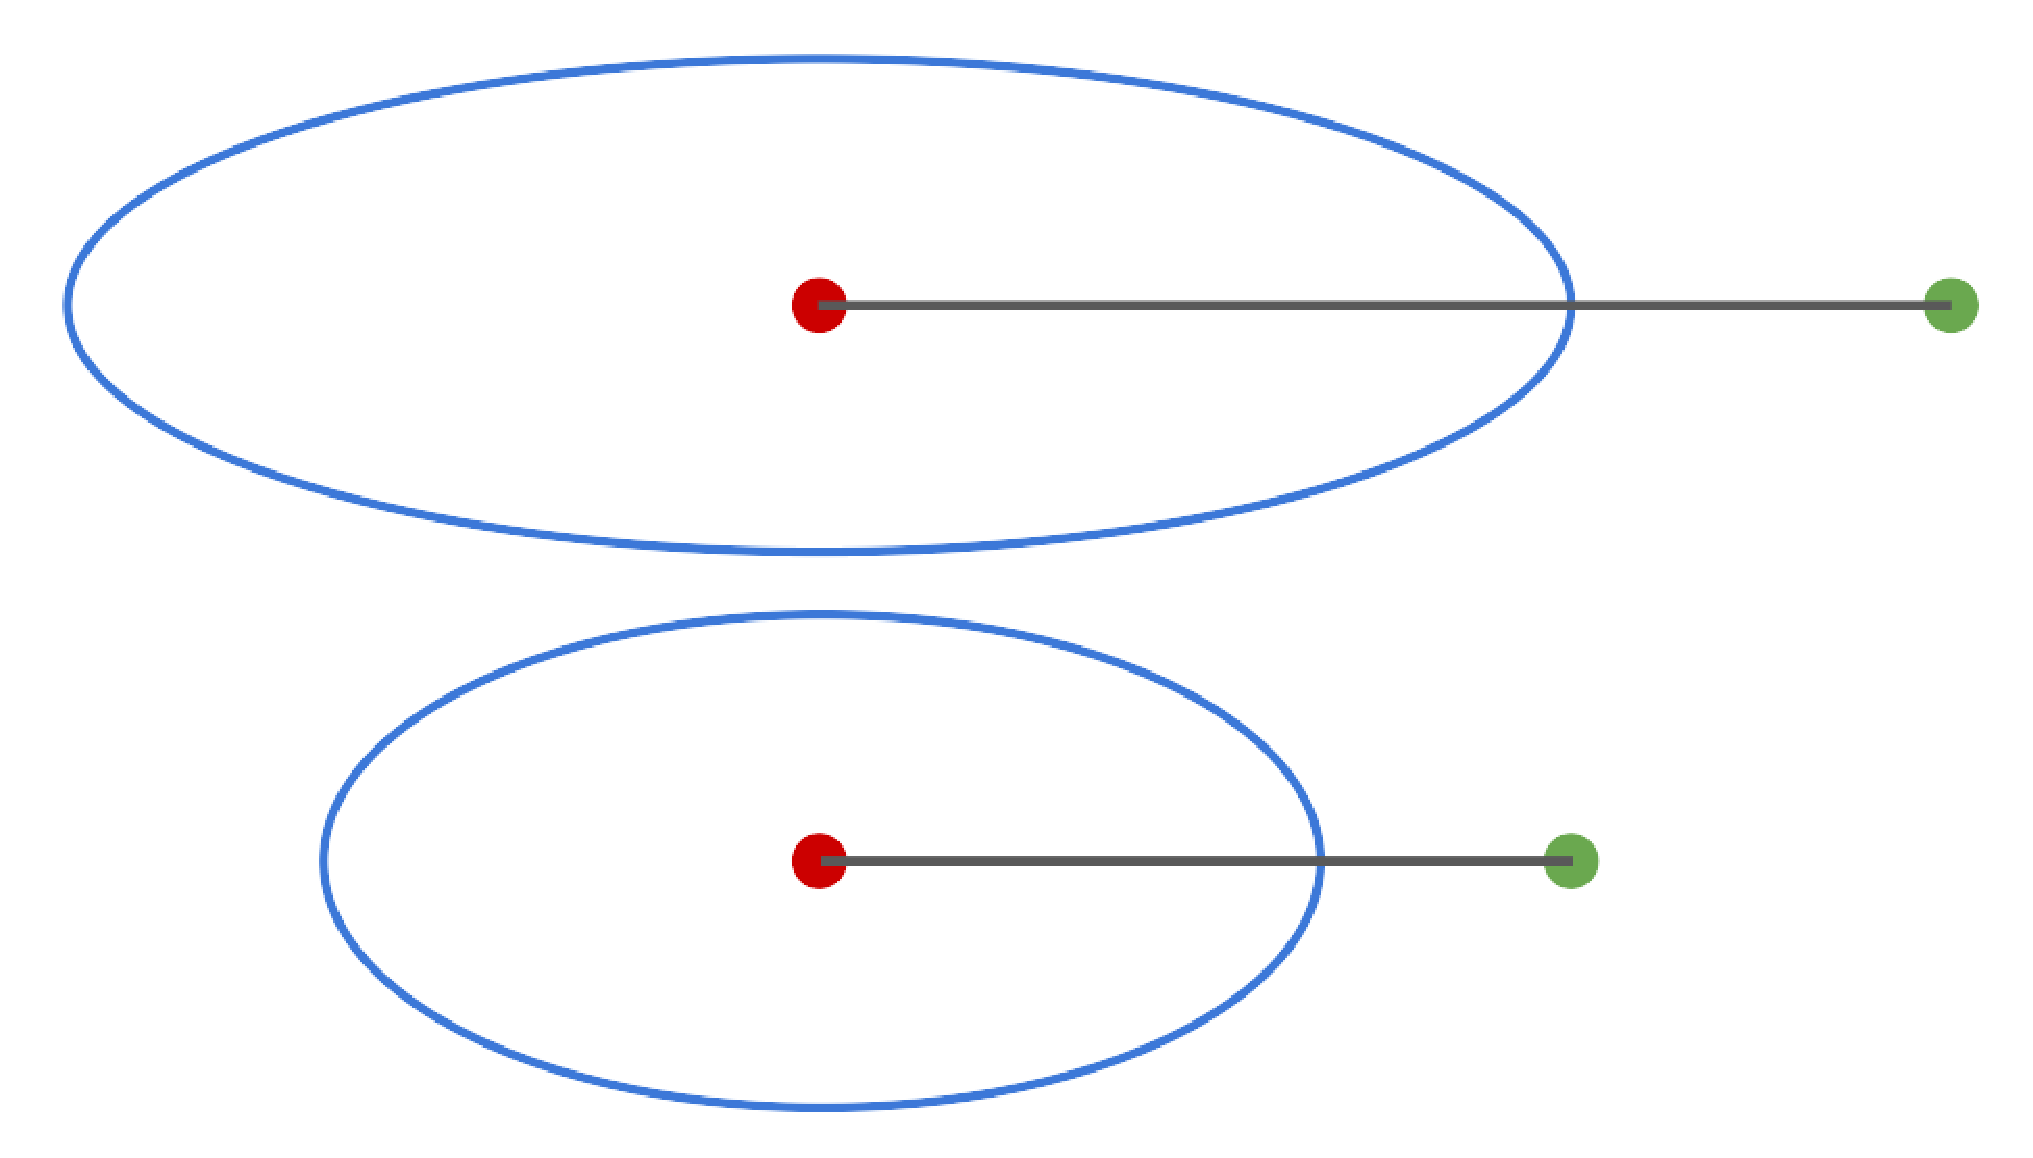
\includegraphics[width=0.75\textwidth]{images/thesis.dispdiagram.eps}
    \caption[Angular Reconstruction Disp]{The disp parameter is the angular distance between the center (red dot) of a hillas image (blue oval) and the reconstructed sky position (green dot).  Generally, longer showers have a larger disp length, while shorter showers have a shorter disp length.}\label{fig:dispdiagram}
  \end{center}
\end{figure}

% https://veritas.sao.arizona.edu/wiki/index.php/BDT_Angular_reconstruction
The disp and other parameters for thousands of simulated showers can then be used to train a neural network that calculates the most probable disp for a given shower.
This most probable disp can then be used with the image axes intersection points to more accurately reconstruct the original gamma-ray point of origin.

Improved angular resolution plot??

\subsection{Energy Reconstruction}\label{subsec:enrecon}
A library of different showers is built, from a variety of elevations, energies, and distances from the camera.
This library can then be used to look up a real shower, find the most similar in elevation, shape, etc, and then reading that shower's library energy.


\section{Sensitivity}
% plot vs energy
Sensitivity is a measure of how difficult it is to get a signifiant detection.
It is often quantified by using simulations to predict the amount of observation time required to detect a simulated source at a given significance level.


\section{Effective Area}
% plot of effective area vs energy
Effective area is the measure of how many gamma rays a telescope can detect.
It is referred to as 'Effective' because the detection efficiency is not 100\% at all energies or all parts of the camera.
Instead it is 'effectivly' how large a detection area a telescope has, if it had perfect detection efficiency.
Different telescopes can use this number to compare roughly how many gamma rays can be detected in a given span of time.


\section{Energy Resolution}
% plot of energy resolution
Gamma rays and protons of different energies can produce similar-looking air showers.
Due to this, the reconstruction software cannot perfectly reconstruct gamma rays, which introduces errors into the different qualities of the gamma rays.
This means that when a gamma ray is reconstructed, it has a chance to be reconstructed at a lower or higher energy.
The consequence of this is that gamma rays of a given reconstructed energy can come from a distribution of true simulated energies.
Typically, simulations are run across a number of energies, and an 2D matrix is assembled, where one axis is the true simulated energy, and the other axis is bins of reconstructed energy.


\section{Point Spread Function}\label{sec:psf}
% plot of psf
In addition to the energy being slightly mis-reconstructed, the source position of the gamma ray can also be misreconstructed.
For a gamma ray telescope, a simple measure of this misreconstruction is to simulate many gamma rays at a single point in the sky, and look at how their reconstructed positions are distributed around that point.
This distribution is referred to as the Point Spread Function.
To first order, most current-generation point spread functions are gaussian distributions.


\section{Energy Dispersion}
Much like the point spread function in section \ref{sec:psf}, the energy reconstruction process is also imperfect.
This means that a gamma ray with a reconstructed energy could come from a distribution of true energies.
This can also be phrased that a group of gamma-rays with the same initial energy will have a distribution of reconstructed energies.
These distributions primarily are due to inherent randomness in the showers themselves.


\section{Energy Sensitivity and Zenith Angle}
% plot of energy sensitivity at 20zen and 65zen

As the telescope points at a lower elevation, the atmospheric volume that can be used to detect air showers greatly increases, leading to an increase in the telescope's effective areafor high energy showers.
The downside is that fewer low-energy gamma rays reach the volume of atmosphere being observed, 


\section{Comparison with Other Observatories}

% sensitivity comparison plots

CTA, HESS, Magic, HAWC, Fermi
